\documentclass[10pt]{article}
\usepackage[T1]{fontenc}
\usepackage[utf8]{inputenc}
\usepackage{mathptmx}
\usepackage[scaled=0.92]{helvet}
\usepackage[a4paper,landscape,margin=1.6cm,top=1.3cm,bottom=1.3cm]{geometry}
\usepackage{graphicx,array,enumitem,tabularx}
\usepackage[table]{xcolor}
\usepackage{fancyhdr}
\pagestyle{fancy}\fancyhf{}\renewcommand{\headrulewidth}{0pt}
\cfoot{\footnotesize Page 1 of 1}
\lfoot{\footnotesize Executive Summary -- Draft for Discussion}
\rfoot{\footnotesize September 2026}
\setlength{\parindent}{0pt}\setlength{\parskip}{4pt}
\newcommand{\hd}[1]{\par\vspace{5pt}{\fontfamily{phv}\selectfont\bfseries\large #1}\par\vspace{1pt}\hrule height 0.6pt\vspace{4pt}}
\begin{document}
\begin{center}
{\fontfamily{phv}\selectfont\bfseries\LARGE Cheaper LLMs as AMR literature screeners}\\[2pt]
{\fontfamily{phv}\selectfont\bfseries\large Executive Summary}\\[4pt]
{\small Hyam Ali \textperiodcentered{} Dr Fabrizio Costa \textperiodcentered{} Dr Shiqiang Wang   \enspace\textbar\enspace   University of Exeter \textperiodcentered{} Google DeepMind Research Ready   \enspace\textbar\enspace   September 2026}
\end{center}
\vspace{-4pt}\hrule height 1.2pt\vspace{1pt}\hrule height 0.4pt
\vspace{6pt}
\textbf{Research question:} Can a cheaper language model stand in for Claude Sonnet 5 when screening PubMed abstracts, without changing which WHO GLASS pathogen--antibiotic pairs come out as research priorities?

\vspace{2pt}
{\renewcommand{\arraystretch}{1.25}
\begin{tabularx}{\linewidth}{|*{5}{>{\centering\arraybackslash}X|}}
\hline
\textbf{\large 89} & \textbf{\large 73,857} & \textbf{\large 711,925} & \textbf{\large 12} & \textbf{\large 2} \\
\small pathogen--antibiotic pairs & \small paper--pair screens & \small LLM decisions & \small models tried & \small acceptance rules \\
\hline
\end{tabularx}}

\vspace{2pt}
\begin{minipage}[t]{0.47\linewidth}
\hd{1.\enspace Key Findings}
\begin{enumerate}[label=\arabic*.,leftmargin=1.6em,itemsep=3pt,topsep=0pt]
\item \textbf{The acceptance rule matters more than which model you use.} Under strict-only, any two candidates put 22--52\% of pairs in different quadrants, compared with just 11--16\% under strict-or-yes. Relaxing the rule helps every model; GPT-3.5, for example, goes from $\rho$ 0.62 to 0.92.
\item \textbf{With the permissive rule, most of the agreement comes from publication volume.} If we skip the LLM entirely and accept every abstract, we still get $\rho$ = 0.95. Gemini 3.5 Flash-Lite (0.97) is the only model that does better, and both GPT models do worse.
\item \textbf{With the strict rule, the choice of model decides the outcome, and even the best one misses emerging pairs.} Gemini 3.5 Flash-Lite reaches $\rho$ 0.87 against 0.67 without an LLM, yet it still moves 38\% of pairs into a different quadrant and finds only 2 of the 13 emerging pairs.
\item \textbf{Agreeing on individual papers is not the same as agreeing on the ranking.} Gemini is the only model with moderate per-paper agreement ($\kappa$ 0.58). Gemma 3 270M is no better than chance ($\kappa$ = $-$0.01), and yet it ranks the pairs at $\rho$ = 0.83.
\end{enumerate}
\vspace{4pt}
\hd{2.\enspace Method}
{\small Every model screened all 73,857 paper--pair items as strict, yes or no. The accepted counts for each pair and year go into a pooled ridge regression, and the residual from that regression is the Scientific Interest (SI) signal. A damped 5-year forecast then puts each pair into a priority quadrant. We compared each model with Sonnet 5 at the paper level (Cohen's $\kappa$) and at the pair level (Spearman $\rho$ and quadrant changes), under the \textbf{strict-only} and \textbf{strict-or-yes} rules and against a \textbf{no-LLM baseline} that accepts every abstract.}
\end{minipage}\hfill
\begin{minipage}[t]{0.49\linewidth}
\hd{3.\enspace Cost versus Fidelity}
\fbox{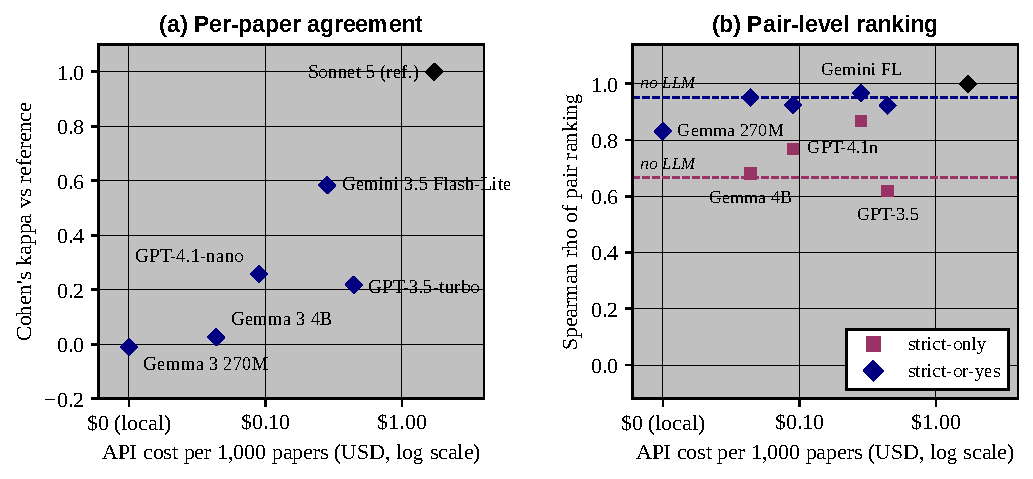
\includegraphics[width=0.975\linewidth]{figs/fig_cost_performance_classic.pdf}}\\[1pt]
{\small\textit{Figure 1.} Agreement with the reference against API cost. Dashed lines mark the no-LLM baseline for each rule. Gemma 3 270M has no strict-only value because its SI signal is constant.}

\vspace{3pt}
{\small\textit{Table 1.} Screening cost by model.}\\[1pt]
{\small\renewcommand{\arraystretch}{1.12}
\begin{tabularx}{\linewidth}{|X|r|r|r|r|}
\hline
\rowcolor[gray]{0.85}\textbf{Model} & \textbf{\$ per 1,000 papers} & \textbf{Full corpus} & \textbf{vs. ref.} & \textbf{Kappa} \\ \hline
Claude Sonnet 5 (ref.) & \$1.72 & \$127.22 & 100\% & 1.00 \\ \hline
Gemini 3.5 Flash-Lite & \$0.28 & \$20.97 & 16\% & 0.58 \\ \hline
GPT-4.1-nano & \$0.09 & \$6.62 & 5\% & 0.26 \\ \hline
GPT-3.5-turbo & \$0.44 & \$32.74 & 26\% & 0.22 \\ \hline
Gemma 3 4B & \$0.04 & \$3.23 & 2.5\% & 0.03 \\ \hline
Gemma 3 270M & \$0.00 & \$0.00 & 0\% & -0.01 \\ \hline
\end{tabularx}}\\[1pt]
{\footnotesize Prices are list prices from Jul--Aug 2026, with Sonnet 5 on the Batch API (50\% off). The full corpus is 73,849 screens. The local model costs \$0 in API fees but took $\sim$84 h on one GPU.}
\end{minipage}

\vfill
\fbox{\parbox{\dimexpr\linewidth-2\fboxsep-2\fboxrule}{\small \textbf{Recommendation.} Gemini 3.5 Flash-Lite is the only substitute that beats the no-LLM baseline under both rules, and it costs 16\% of the reference (\$21 against \$127 for the full corpus). The acceptance rule should be reported as a main design choice, and any strict-or-yes result should be compared with the no-LLM baseline.\\[3pt]
\textbf{Before submission:} we still have no human ground truth, and 6.6\% of the reference screens came back empty (probably because adaptive thinking hit the 60-token cap), so these need re-running. The work also rests on a single prompt, and the size ladder covers only 3 of the 89 pairs.}}
\end{document}
